\documentclass[../main.tex]{subfiles}

\begin{document}
\doublespacing

% \begin{table}[H]
% \centering
% \resizebox{\textwidth}{!}{%
% \begin{tabular}{@{}cllll@{}}
% \toprule
% \textbf{\begin{tabular}[c]{@{}c@{}}Initial Temperature\\ $(\si{\celsius})$\end{tabular}} & \multicolumn{1}{c}{\textbf{\begin{tabular}[c]{@{}c@{}}Mass of Salt\\ $(\si{\gram})$\end{tabular}}} & \multicolumn{1}{c}{\textbf{\begin{tabular}[c]{@{}c@{}}Volume of Sample\\ $(\si{\milli\liter})$\end{tabular}}} & \multicolumn{1}{c}{\textbf{\begin{tabular}[c]{@{}c@{}}Concentration\\ $()$\end{tabular}}} & \multicolumn{1}{c}{\textbf{\begin{tabular}[c]{@{}c@{}}Elapsed Time until $\SI{0}{\celsius}$\\ $(\si{\second})$\end{tabular}}} \\ \midrule % End of Header
% &   & $0$  &   & \\
% &   & $1$  &   & \\                                                                                                                              
% &   & $2$  &   & \\
% &   & $3$  &   & \\
% &   & $4$  &   & \\
% &   & $5$  &   & \\\bottomrule
% \end{tabular}%
% }
% \caption{}
% \label{tab:my-table}
% \end{table}

As from Table~\ref{tab:28Table} and Table~\ref{tab:50Table}, Mpemba effect was not observed for the control samples (\SI{0}{\milli\gram\per\milli\liter}). The time taken for the cooler sample to reach $\SI{0}{\celsius}$ was $\SI{2030}{\second}$ whereas the hotter sample took $\SI{2980}{\second}$. \textbf{This shows that the initially cooler water did indeed reach $\SI{0}{\celsius}$ before the initially hotter water.}   \par 

Results further show that for both initial temperatures $T_i$ (\SI{28}{\celsius} and \SI{50}{\celsius}), increasing the mass concentration of salt, $\rho_i$, from $0$ to $\SI{125}{\milli\gram\per\liter}$, resulted in a decreases of the elapsed time until the samples reached $\SI{0}{\celsius}$. In particular, the \SI{2030}{\second} to \SI{1940}{\second} (for $T_i = \SI{28}{\celsius}$), as shown in Table \ref{tab:28Table}, and from \SI{2980}{\second} to \SI{1950}{\second} (for $T_i = \SI{50}{\celsius}$) noted in Table \ref{tab:50Table}. \par

Accounting for the anomalies shown in bold, it should be noted that those samples appear to be out of the proposed trend. In those cases, it might be proposed that the samples supercooled and were thus able to cool faster. However, in both cases in Table~\ref{tab:28Table} and Table~\ref{tab:50Table}, those behaviors occur without a particular pattern which further reinstates that it might be an oddity that is best understood through the supercooling behavior of water. \par

\begin{table}[H]
\centering
\renewcommand{\arraystretch}{1.2}
\resizebox{\textwidth}{!}{%
\begin{tabular}{@{}ccccc@{}}
\toprule
\textbf{\begin{tabular}[c]{@{}c@{}}Initial Temperature \\ $T_i$ $(\si{\celsius})$\end{tabular}} & \textbf{\begin{tabular}[c]{@{}c@{}}Mass of Salt \\ $m$ $(10^3 \, \si{\milli\gram})$\end{tabular}} & \textbf{\begin{tabular}[c]{@{}c@{}}Volume of Sample \\ $V$ $(\si{\milli\liter})$\end{tabular}} & \textbf{\begin{tabular}[c]{@{}c@{}}Mass Concentration \\ $\rho_i$ $(\si{\milli\gram\per\milli\liter})$\end{tabular}} & \textbf{\begin{tabular}[c]{@{}c@{}}Elapsed Time until $\SI{0}{\celsius}$ \\ $t$ $(\si{\second})$\end{tabular}} \\ \midrule
\multirow{6}{*}{$28$}                                                                           & $0$                                                                                               & \multirow{6}{*}{$40$}                                                                          & $0$                                                                                                                  & 2030                                                                                                           \\
                                                                                                & $1$                                                                                               &                                                                                                & $25 \pm 0.563 $                                                                                                       & 2020                                                                                                            \\
                                                                                                & $2$                                                                                               &                                                                                                & $50 \pm 0.875$                                                                                                        &$2000$                                                                                                              \\
                                                                                                & $3$                                                                                               &                                                                                                & $75 \pm 1.19$                                                                                                        & $\mathbf{1940}$                                                                                                              \\
                                                                                                & $4$                                                                                               &                                                                                                & $100 \pm 1.50$                                                                                                       & $1990$                                                                                                             \\
                                                                                                & $5$                                                                                               &                                                                                                & $125 \pm 1.81$                                                                                                       & 1940                                                                                                           \\ \bottomrule
\end{tabular}%
}
\caption{Data collected for initial temperature $T_i = \SI{28}{\celsius}$. Anomalies are shown in bold}
\label{tab:28Table}
\end{table}

\begin{table}[H]
\centering
\renewcommand{\arraystretch}{1.2}
\resizebox{\textwidth}{!}{%
\begin{tabular}{@{}ccccc@{}}
\toprule
\textbf{\begin{tabular}[c]{@{}c@{}}Initial Temperature \\ $T_i$ $(\si{\celsius})$\end{tabular}} & \textbf{\begin{tabular}[c]{@{}c@{}}Mass of Salt \\ $m$ $(10^3 \, \si{\milli\gram})$\end{tabular}} & \textbf{\begin{tabular}[c]{@{}c@{}}Volume of Sample \\ $V$ $(\si{\milli\liter})$\end{tabular}} & \textbf{\begin{tabular}[c]{@{}c@{}}Mass Concentration \\ $\rho_i$ $(\si{\milli\gram\per\milli\liter})$\end{tabular}} & \textbf{\begin{tabular}[c]{@{}c@{}}Elapsed Time until $\SI{0}{\celsius}$ \\ $t$ $(\si{\second})$\end{tabular}} \\ \midrule
\multirow{6}{*}{$50$}                                                                           & $0$                                                                                               & \multirow{6}{*}{$40$}                                                                          & $0$                                                                                                                  & $2980$                                                                                                         \\
                                                                                                & $1$                                                                                               &                                                                                                & $25 \pm 0.563 $                                                                                                       & $2670$                                                                                                              \\
                                                                                                & $2$                                                                                               &                                                                                                & $50 \pm 0.875$                                                                                                        & $\mathbf{2100}$                                                                                                              \\
                                                                                                & $3$                                                                                               &                                                                                                & $75 \pm 1.19$                                                                                                        & $2360$                                                                                                              \\
                                                                                                & $4$                                                                                               &                                                                                                & $100 \pm 1.50$                                                                                                       & $2170$                                                                                                              \\
                                                                                                & $5$                                                                                               &                                                                                                & $125 \pm 1.81$                                                                                                       & $1950$                                                                                                         \\ \bottomrule
\end{tabular}%
}
\caption{Data collected for initial temperature $T_i = \SI{50}{\celsius}$. Anomalies are shown in bold.}
\label{tab:50Table}
\end{table}

Further comparing the elapsed times until $\SI{0}{\celsius}$ between Table \ref{tab:28Table} and \ref{tab:50Table}, we may note that the Mpemba effect was not observed for any mass concentration, as all initially cooler samples cooled down to \SI{0}{\celsius} first. However, it should be noted that for the concentration of $\SI{125}{\milli\gram\per\milli\liter}$, the effect was very close to being observed. In fact, while the cooler sample reached $\SI{0}{\celsius}$ in $\SI{1940}{\second}$, the initially hotter sample reached it in $\SI{1950}{\second}$, with a mere $\SI{10}{\second}$ difference. \par

\begin{figure}[H]
    \centering
    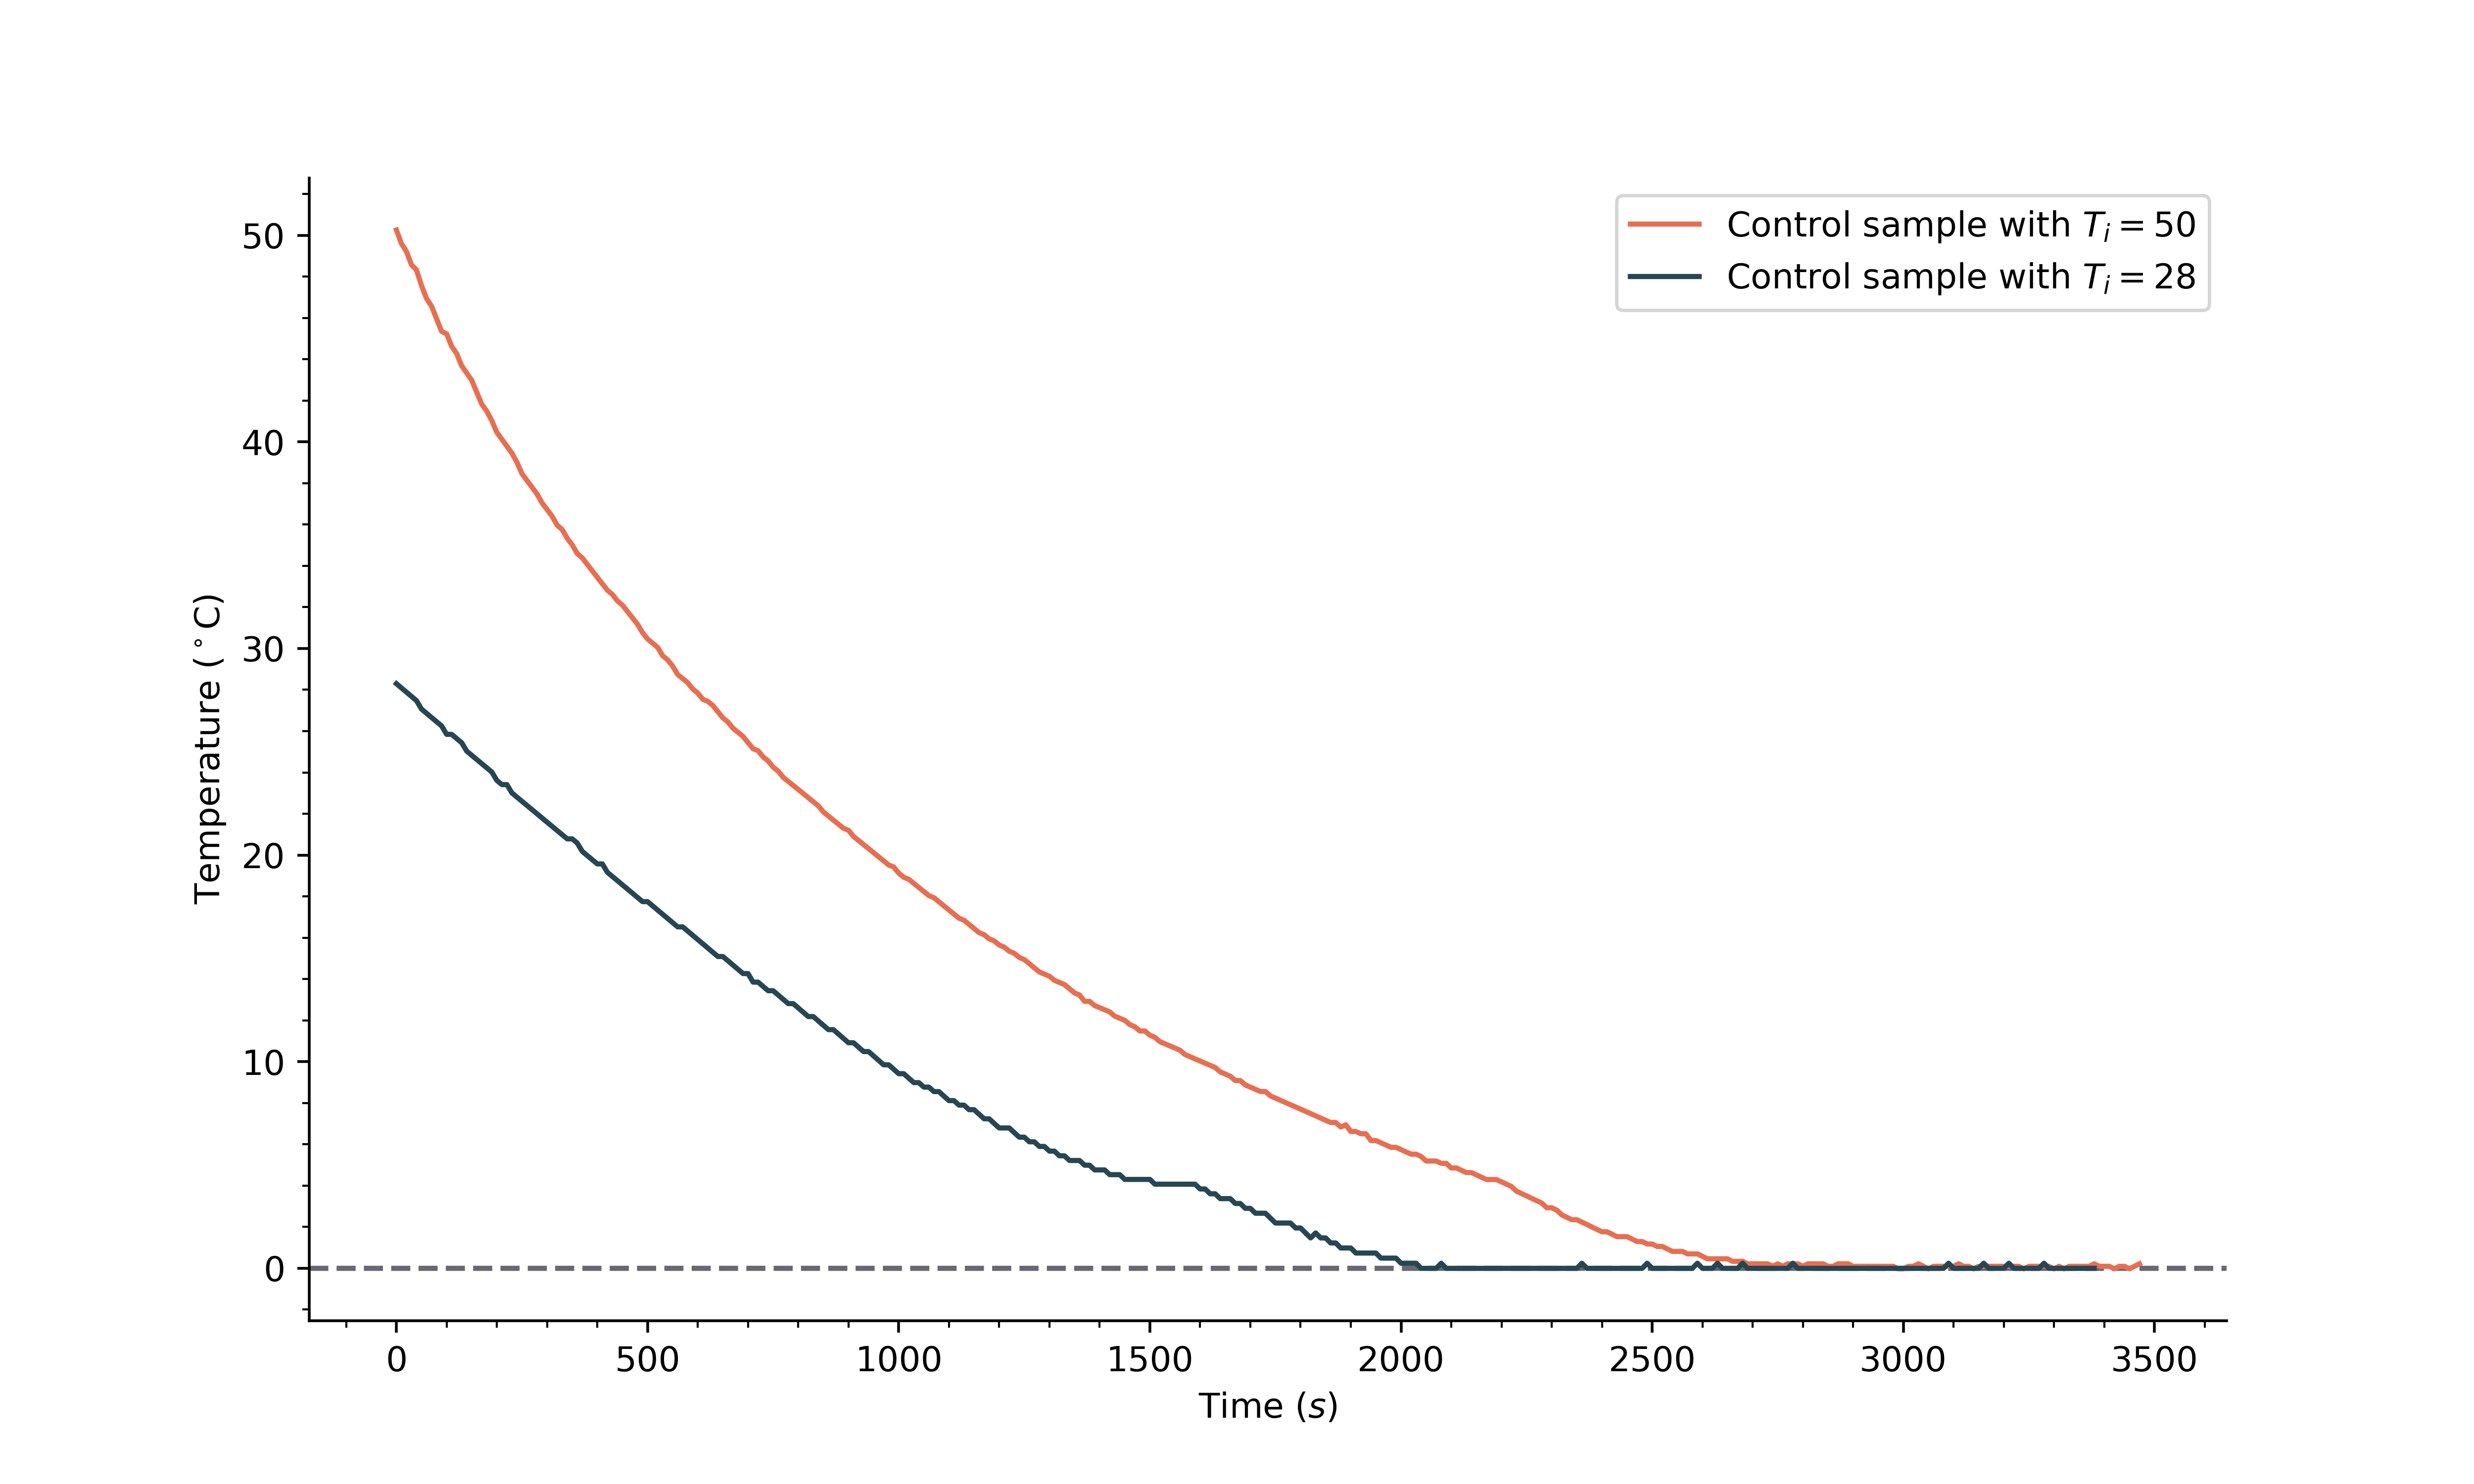
\includegraphics[scale=0.6]{figures/controlSamples.png}
    \caption{Control samples at $T_i = \SI{50}{\celsius}$ (orange) and $T_i = \SI{28}{\celsius}$ (blue).}
    \label{fig:controlSamples}
\end{figure}

Although $\SI{125}{\milli\gram\per\milli\liter}$ did not observe the Mpemba effect, their behavior below $\SI{0}{\celsius}$ was very different from the rest. As seen in Fig.~\ref{fig:5GSamples}, initially hotter sample reached the colder temperatures before the initially cooler sample. This behavior was also observed by \textcite{ibekwe_investigating_2016} for similar group samples, whereby they claimed to have observed the Mpemba effect. It is worth noting that both \textcite{ibekwe_investigating_2016} and \textcite{jeng_mpemba_2006} chose the point where the ice forms as the freezing point. This study considered the point $\SI{0}{\celsius}$ as the freezing point for all samples, for the sake of repeatability and in order to be more in line with the original research done by \textcite{mpemba_cool_1969}. \par

In comparison to the control samples (Fig. \ref{fig:controlSamples}), samples with \SI{125}{\milli\gram\per\milli\liter} (Fig. \ref{fig:5GSamples}) exhibited a significantly different behavior. Whereas the two \SI{125}{\milli\gram\per\milli\liter} samples reached the \SI{2000}{\second} mark at approximately the same time; temperature curves of the control samples continued running parallel during the duration of the experiment, with cooler sample reaching \SI{0}{\celsius} first. \par

\begin{figure}[H]
    \centering
    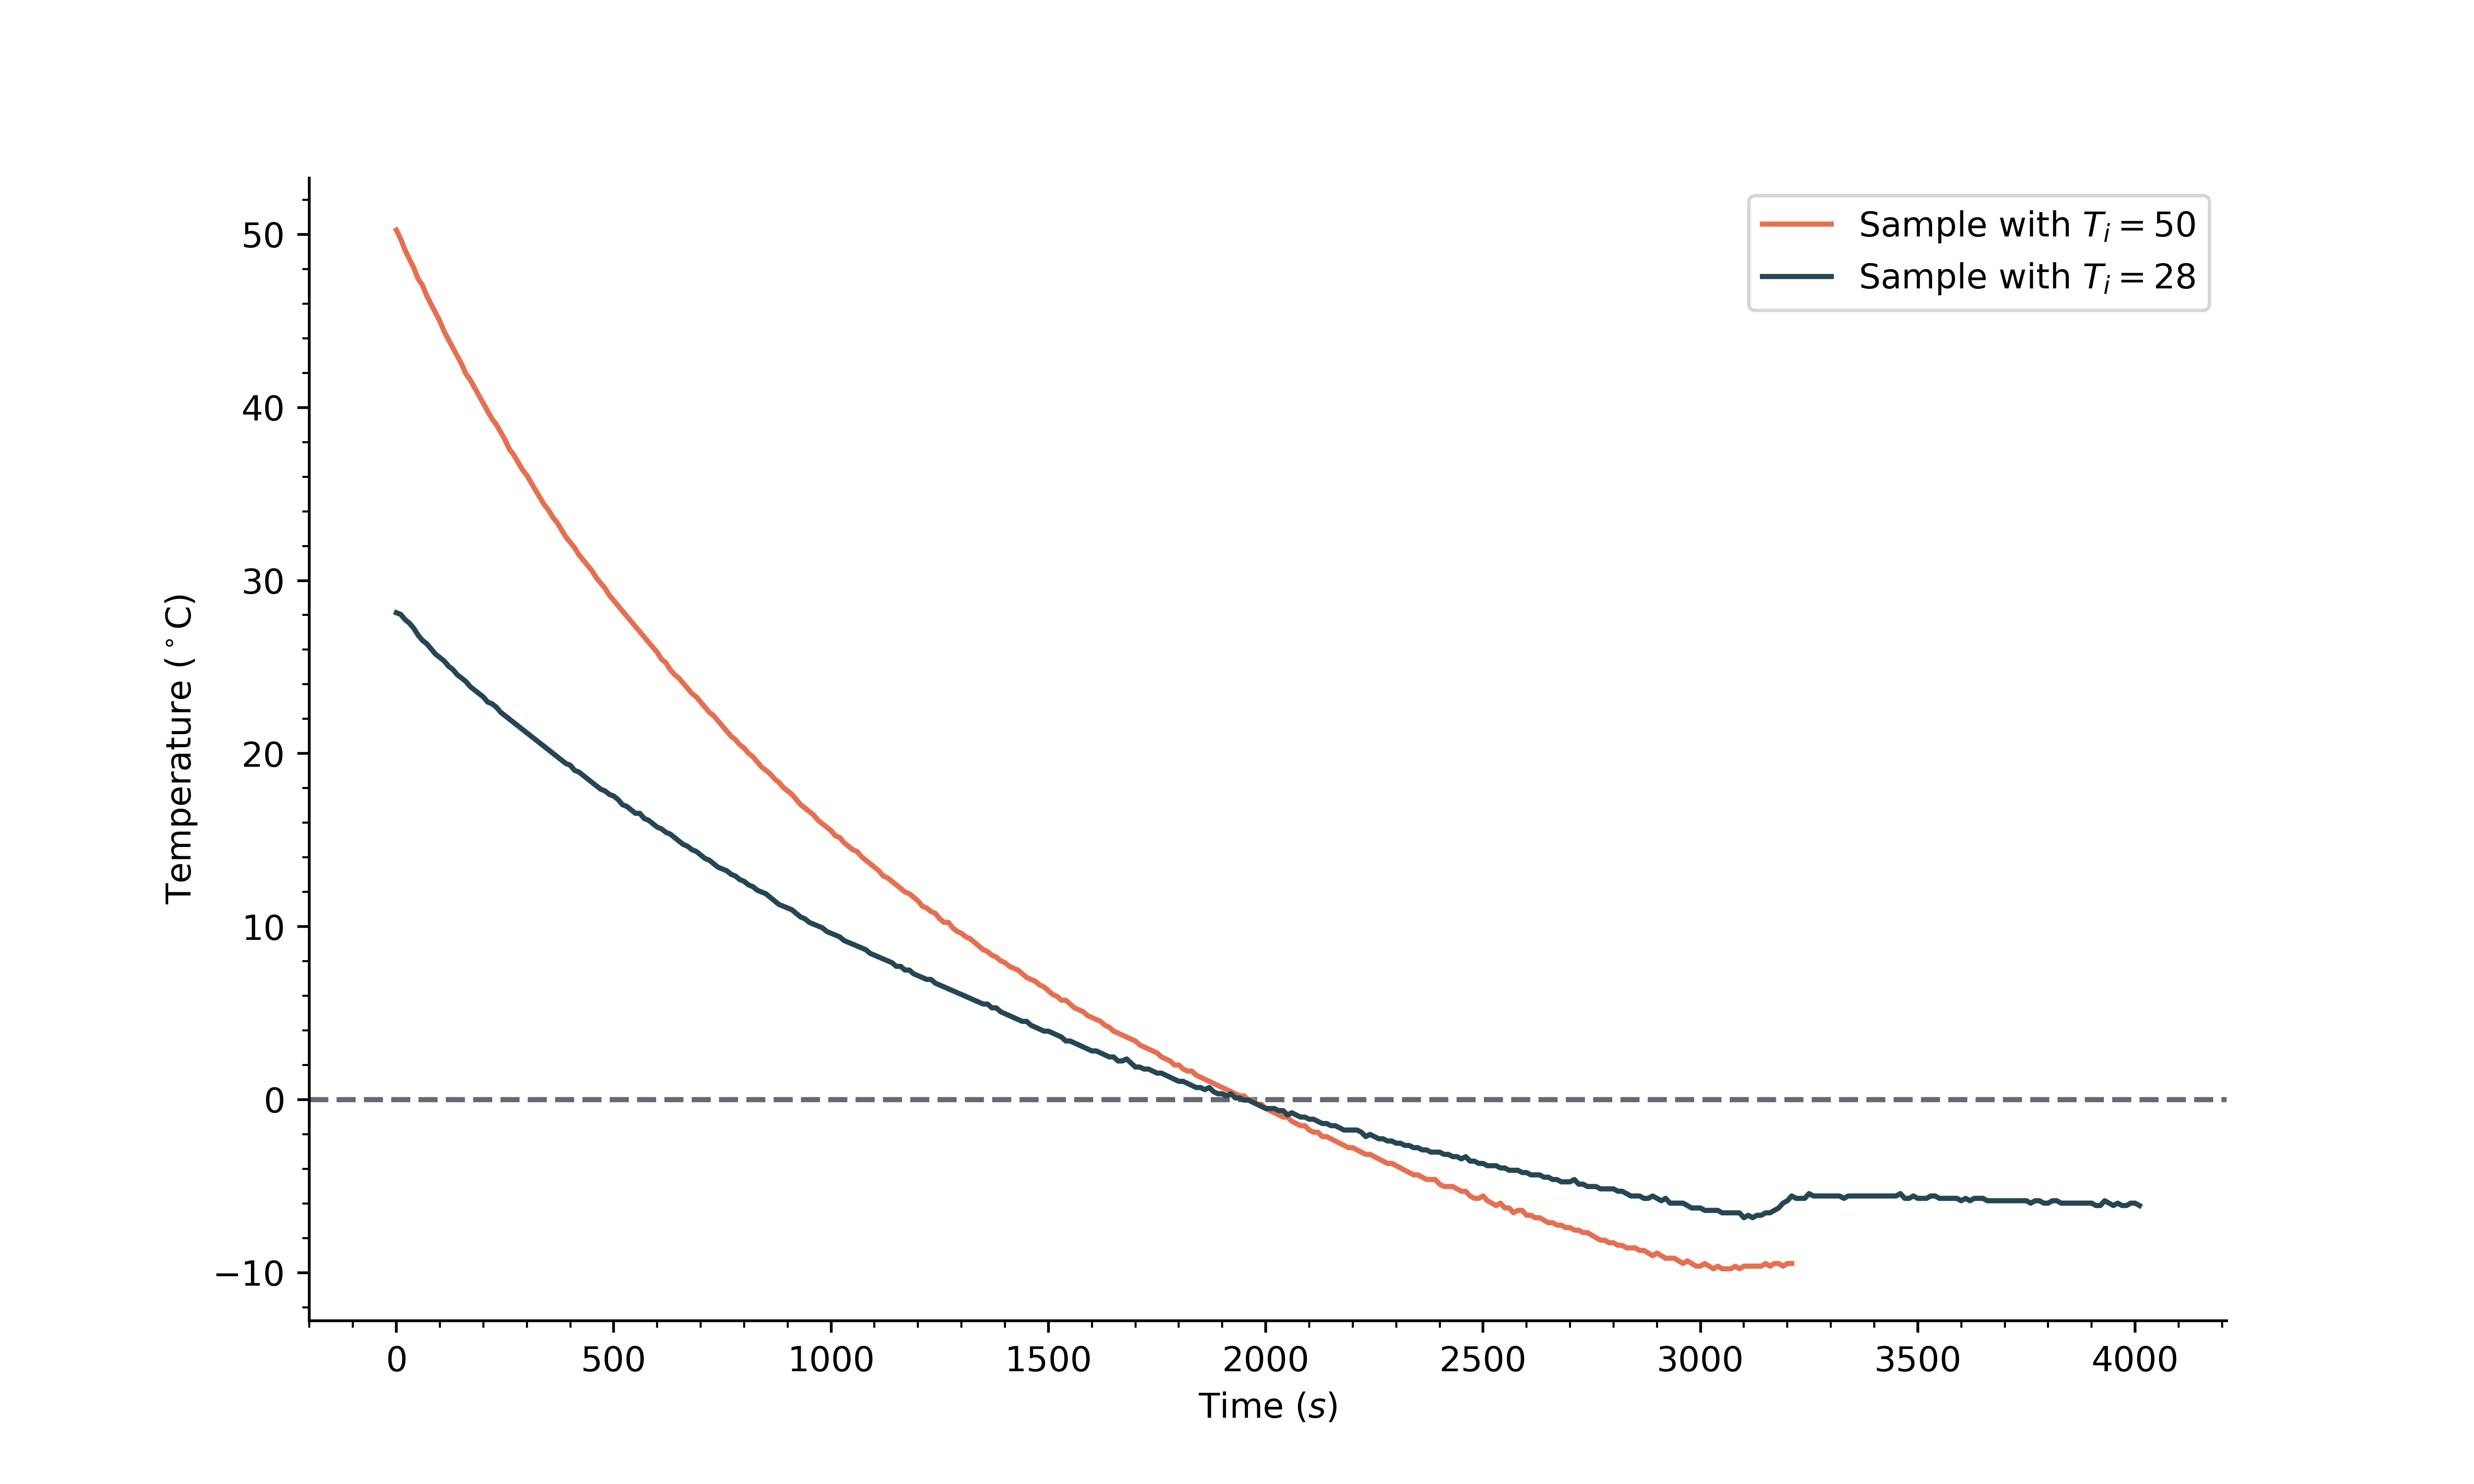
\includegraphics[scale=0.6]{figures/5GSamples.png}
    \caption{$\SI{5}{g}$ samples at $T_i = \SI{50}{\celsius}$ (orange) and $T_i = \SI{28}{\celsius}$ (blue).}
    \label{fig:5GSamples}
\end{figure}

Overall, the salted samples were observed to have lower freezing temperatures as compared to the control samples. Furthermore, this implied that the rate of change of temperature for salted samples was greater and thus resulted in steeper temperature curve. Conversely, gradients for the control samples were observed to be less steep for the same reasons. \par

Furthermore, it was noted that the time taken for the hotter sample took only $0.515\% $ more time to reach \SI{0}{\celsius} in comparison to the cooler sample. \textcite{ibekwe_investigating_2016} observed a difference of $14\%$ between hotter sample freezing first and cooler sample freezing afterwards.

In addition, as noted by \textcite{jeng_mpemba_2006}, "Finding that the Mpemba effect does not occur under certain conditions is a good experimental result." In another study by \textcite{ibekwe_investigating_2016} it was claimed that the convection currents circulate the warmest water to the surface, accelerating these mechanisms and that above approximately $\SI{45}{\celsius}$ they are sufficiently accelerated to enable a body of water to overtake a cooler body of water, reaching $\SI{0}{\celsius}$ and freezing first. In comparison with the theory of solutes, the convection currents might offer a valid explanation to the observed processes. \par 

% \begin{figure}
%     \centering
%     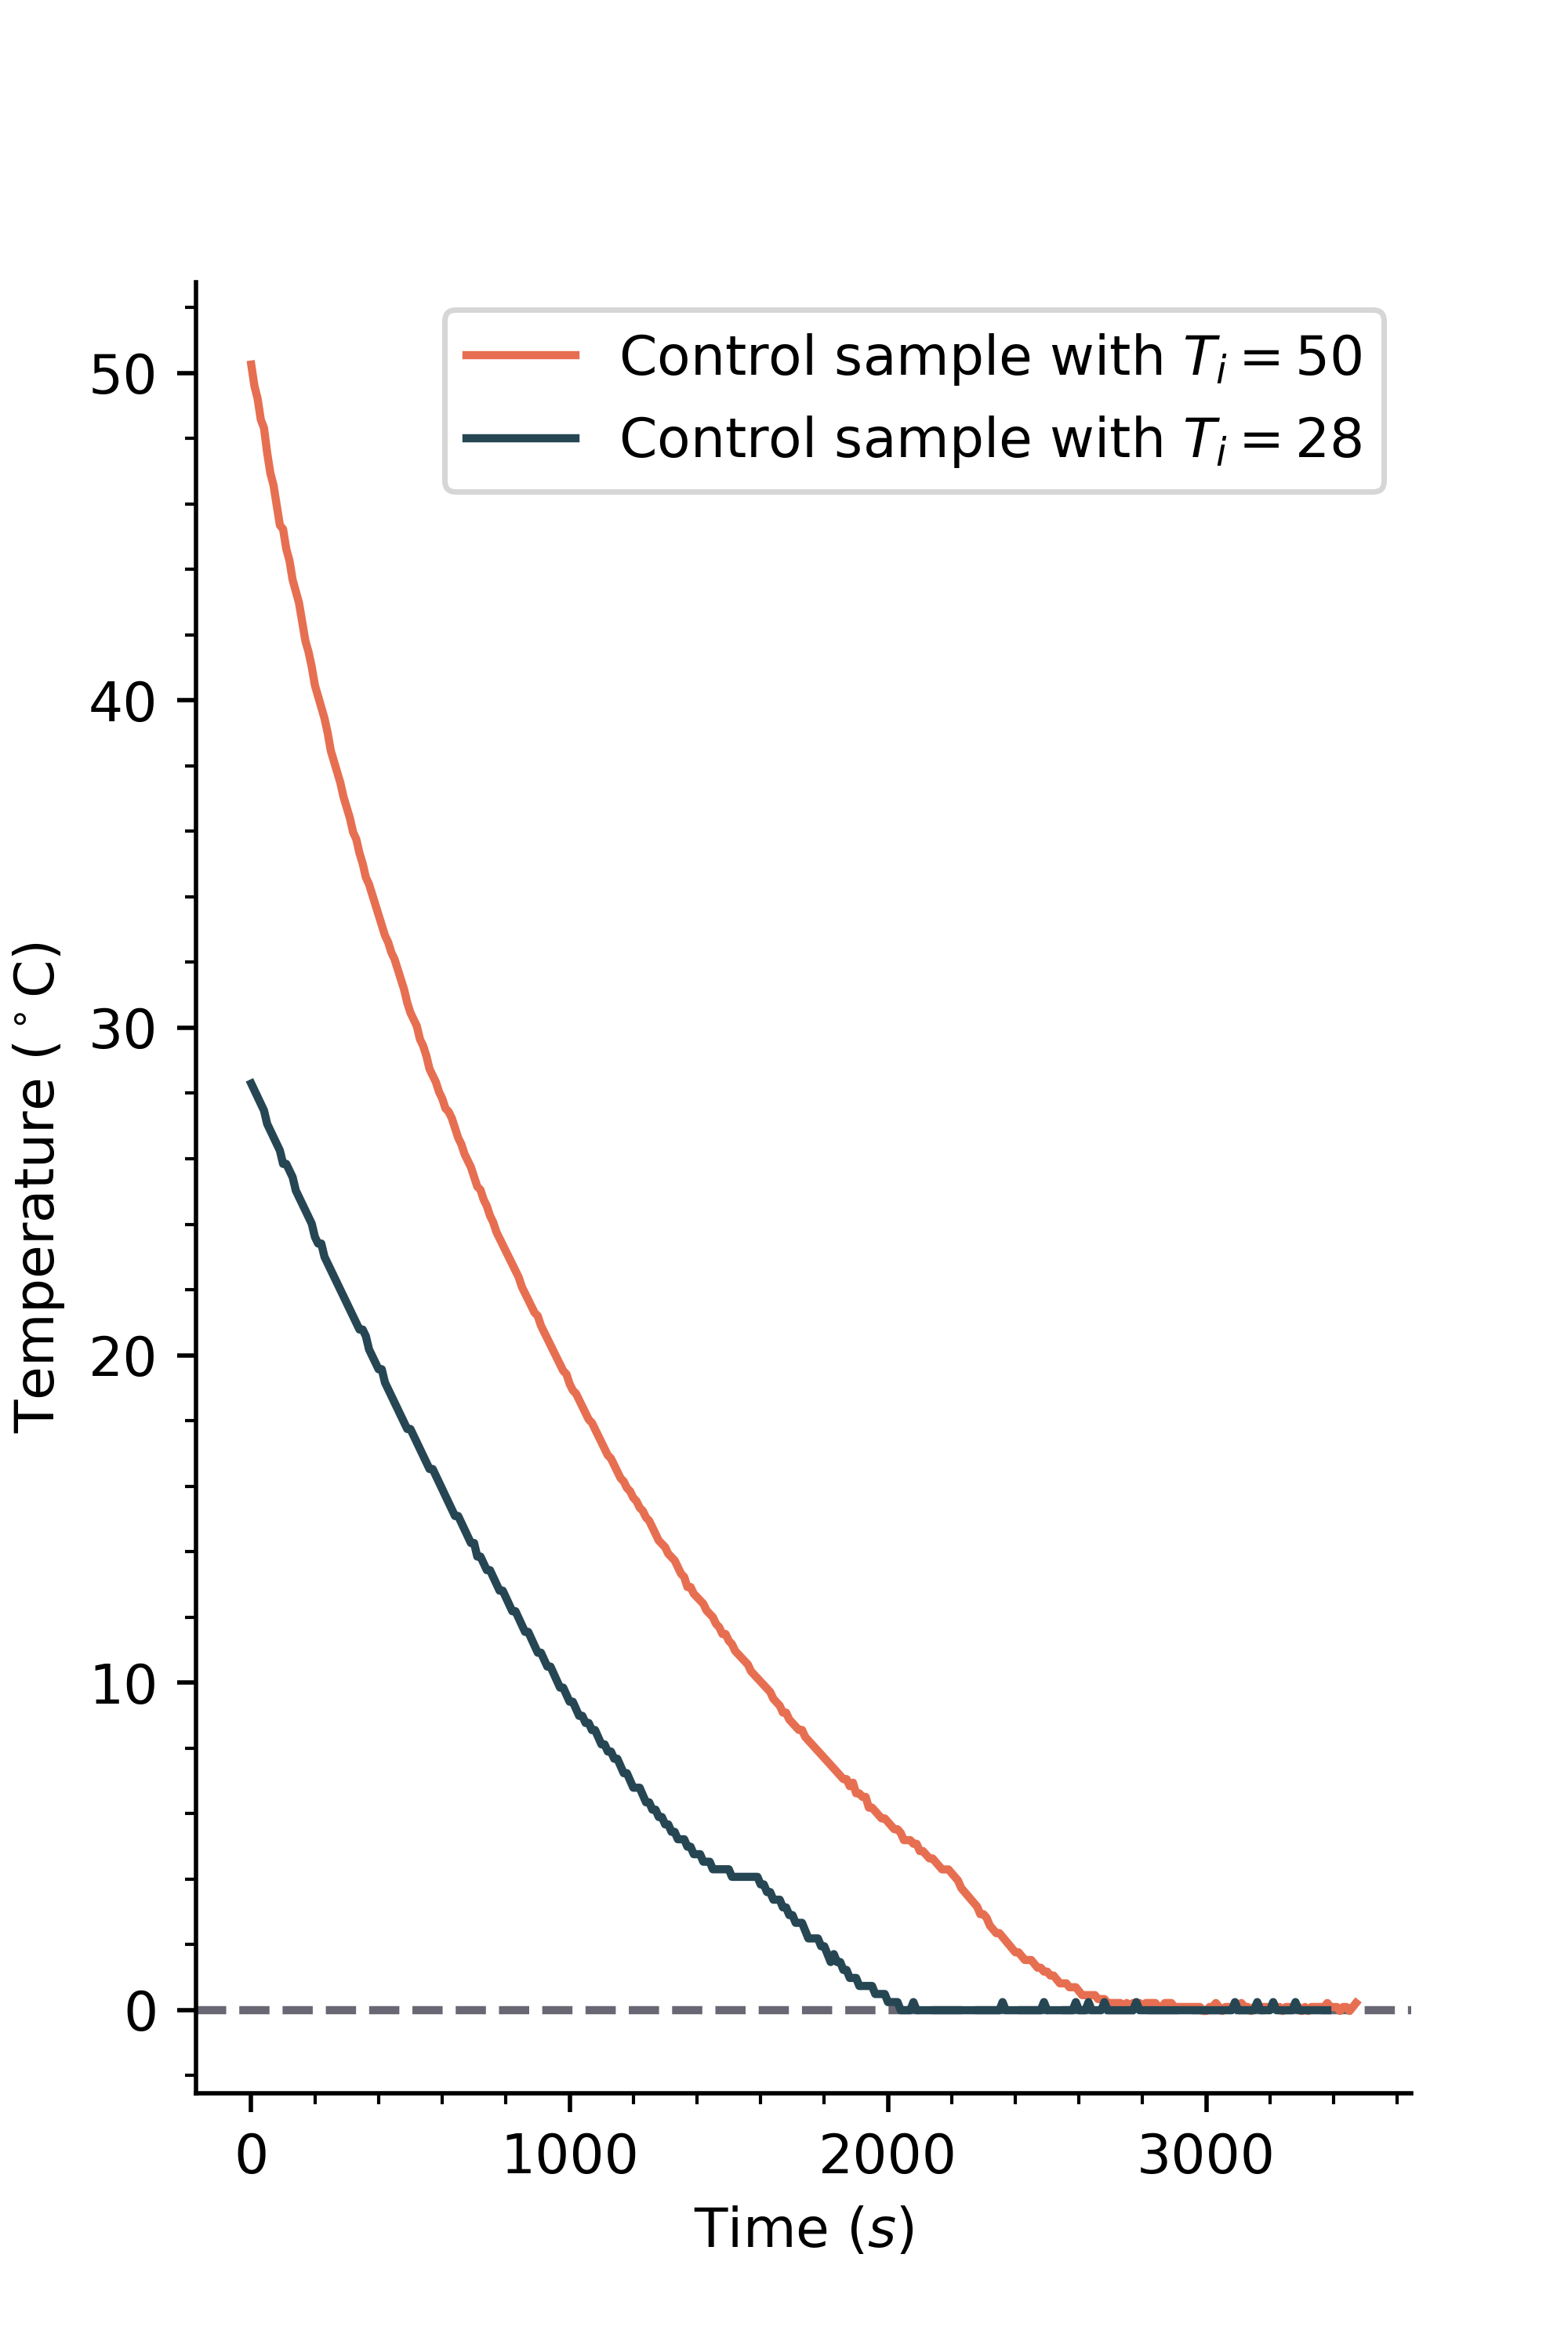
\includegraphics[scale = 0.7]{figures/figureTwo.png}
%     \caption{Caption}
%     \label{fig:my_label}
% \end{figure}

% \begin{figure}[H]
%   \begin{subfigure}{0.49\textwidth}
%     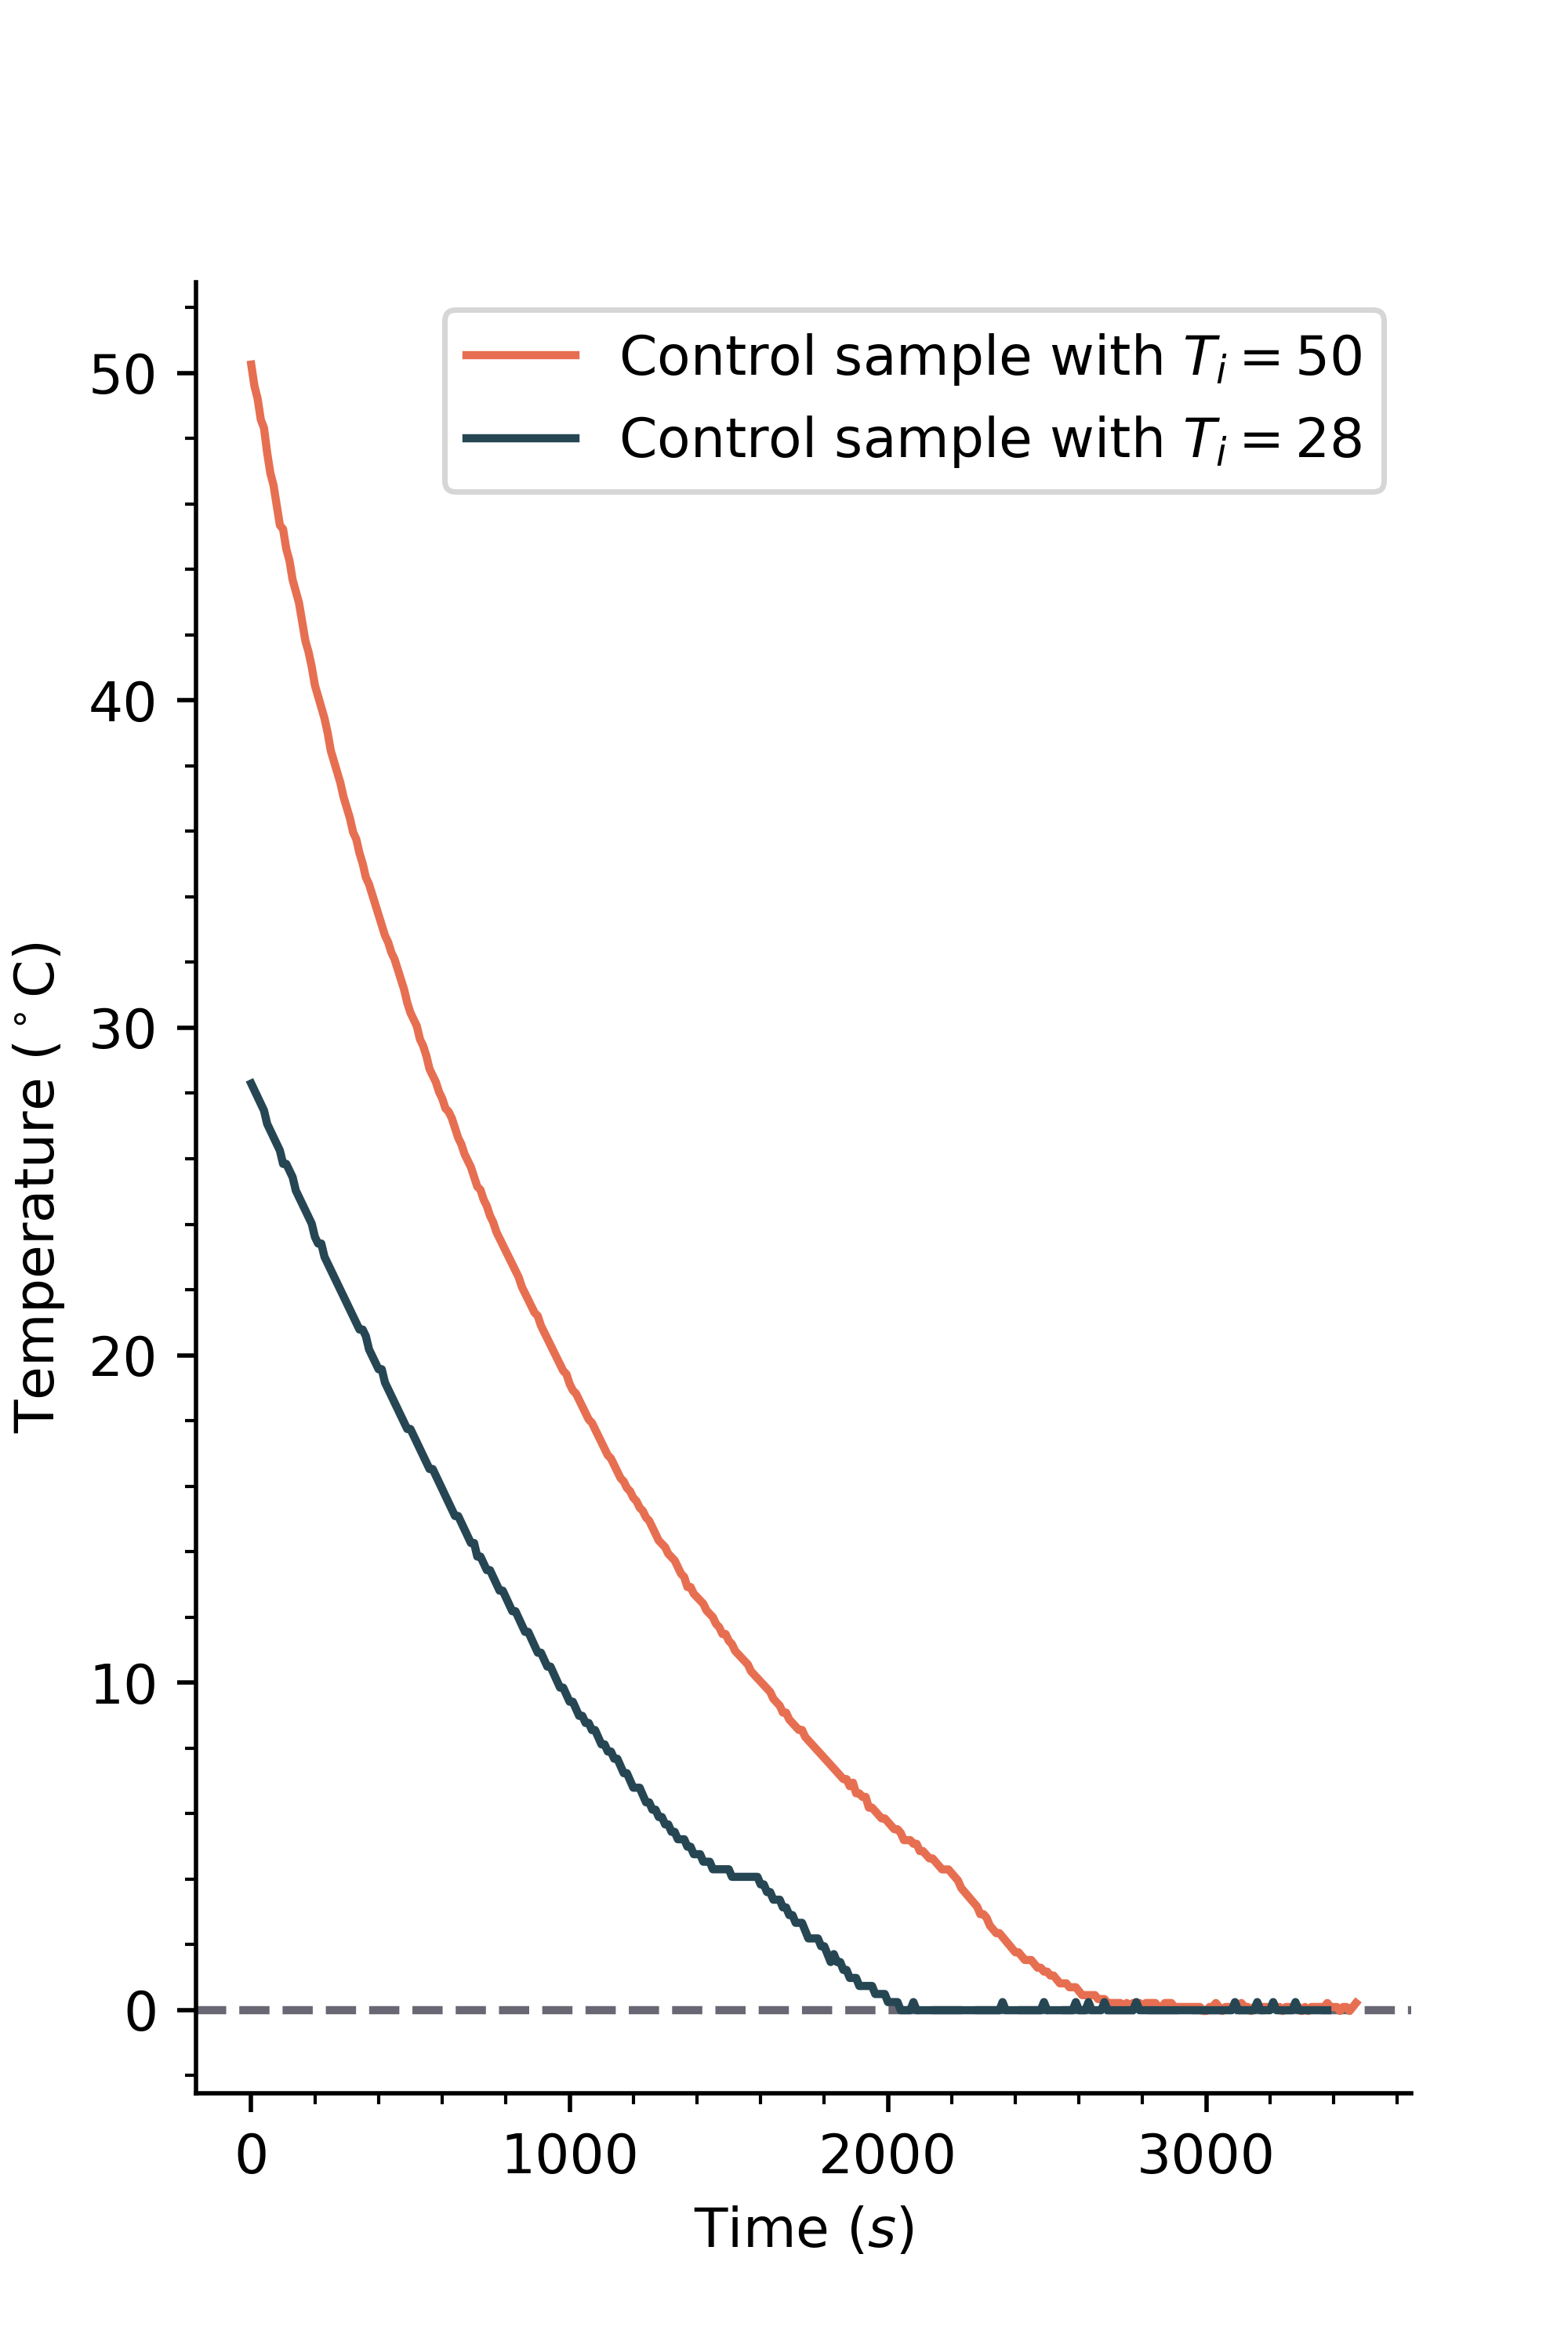
\includegraphics[width=\linewidth]{figures/figureTwo.png}
%     \caption{Function $f(x)$ and polynomial $P(x)$ where $\deg(P(x)) = 0$.} \label{fig:taylorOne}
%   \end{subfigure}%
%   \hspace*{\fill}   
%   \begin{subfigure}{0.49\textwidth}
%     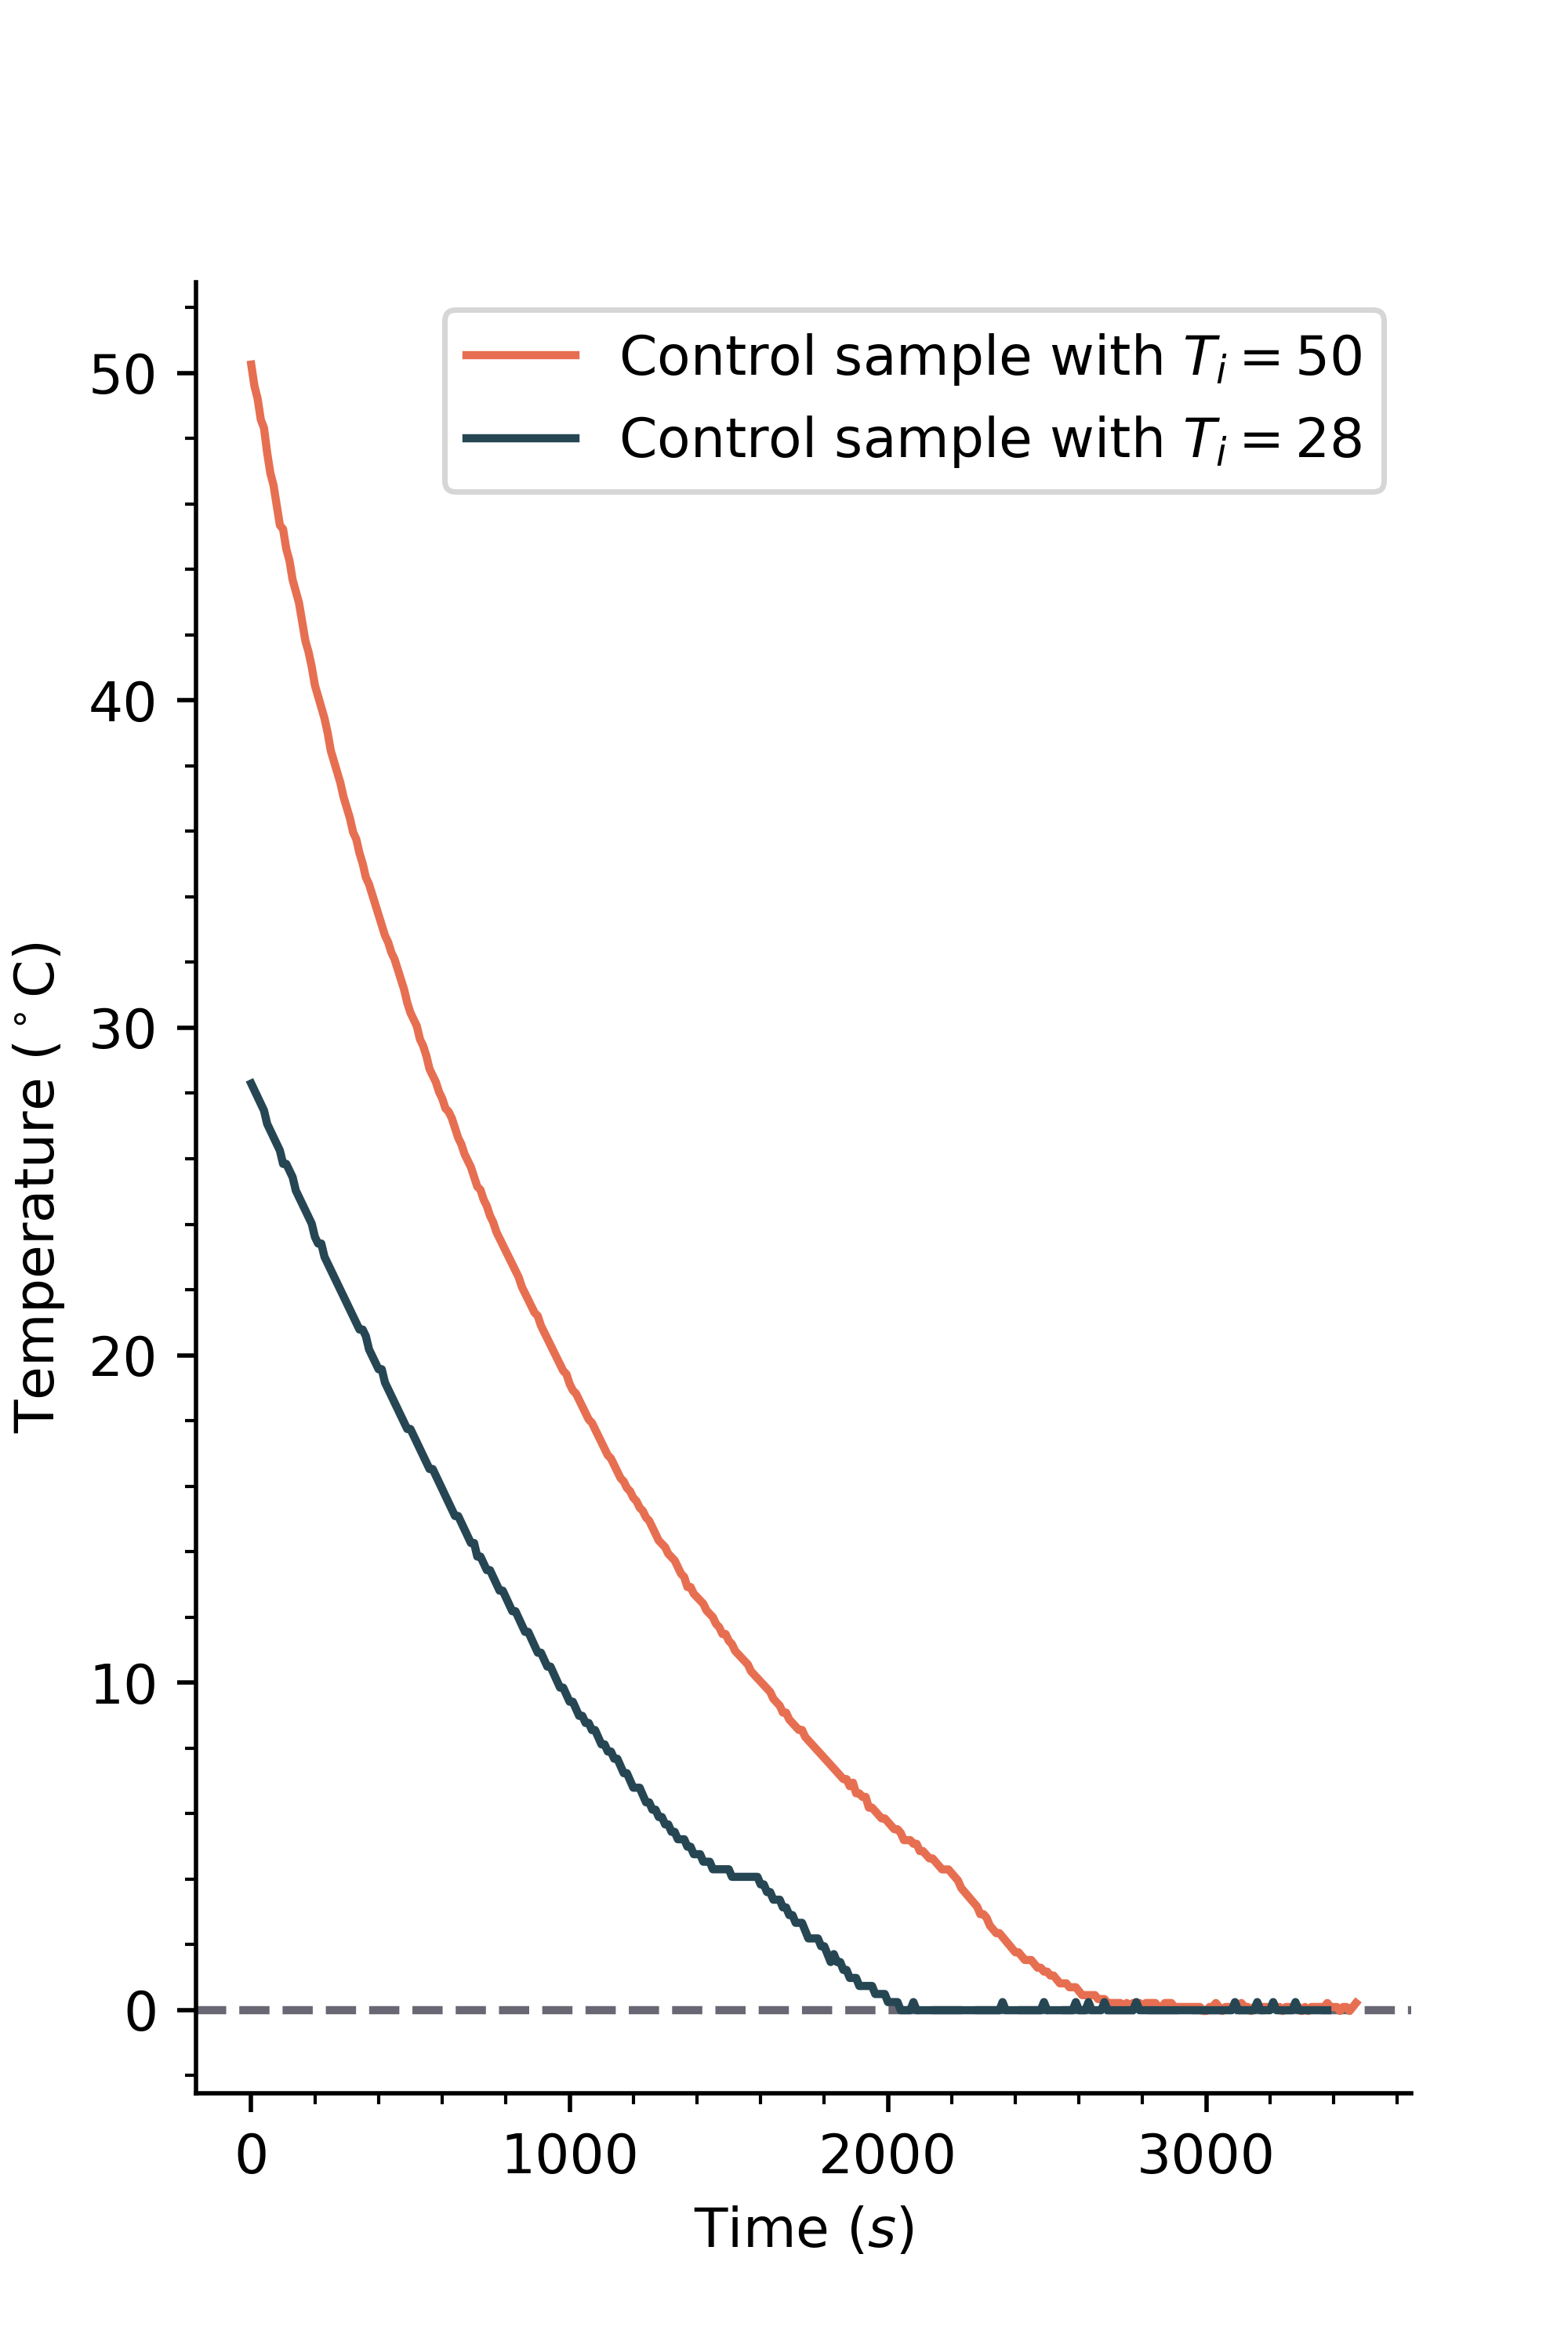
\includegraphics[width=\linewidth]{figures/figureTwo.png}
%     \caption{Function $f(x)$ and polynomial $P(x)$ where $\deg(P(x)) = 1$.} \label{fig:taylorTwo}
%   \end{subfigure}%
% \caption{Approximating $f(x) = e^x$ with polynomial $P(x)$} \label{fig:taylorApprox}
% \end{figure}

% Consider comparing 50 C temp with 30 C temp for every trial


\end{document}